\chapter[ GPGPU-Based Implementation of a finite difference algorithm]{GPGPU-Based Implementation of \\ a finite difference algorithm}

\label{CHAPTER:CUDA}

The objective of this chapter is to give an overview of the basic implemenation of an algorithm using finite difference schemes.
The source code used for the computations is based on an existing and validated version from A. Tilgner.
It was furthermore extended by the immersed boundary methods, which will be explained in more detail in chapter \ref{CHAPTER:IBM}.
In this context an introduction to the aspects of GPGPU\footnote{General Purpose Computation on Graphics Processing Uni}-Computing
with the CUDA \footnote{Computing Uniform Device Architecture} architecture will be given.
For the computations in this thesis Tesla C1060 and Tesla K20m GPUs by NVIDIA were used.%, the complete system configurations can be looked up at (AX.X).
In this chapter, all informations related to GPGPU-Computing and CUDA are adapted from the CUDA Programming Guide and the CUDA Best Practices Guide from NVIDIA
\citep{CUDAPG}, \citep{CUDABP}. All details about the implementation of the algorithm were obtained by studying the source code
and from private communication with A.Tilgner.

\section{GPGPU-Computing with CUDA}

CUDA is an architecture developed by NVIDIA to enable an easy approach to the implementation of GPGPU-based algorithms.
The underlying idea is to hide the complexity of the hardware under a more high oriented and generalized software abstraction layer.
This is done by introducing some additional programming language extensions for example in C/C++,
furthermore it is necessary to use a CUDA suited compiler like NVCC.

\subsection{Hardware and Memory Architecture}

A cuda device contains an array of so called streaming multiprocessors (SM).
Each of these SMs contains a group of small execution units, which are called cuda cores.
For the exchange of data between different SMs, cuda cores and the CPU side of the computer, there exists different
types of memory, as shown  in Fig.  \ref{fig:gpu_memory_layout}.
\newpage

\begin{figure}[!tbp]
      \centering
        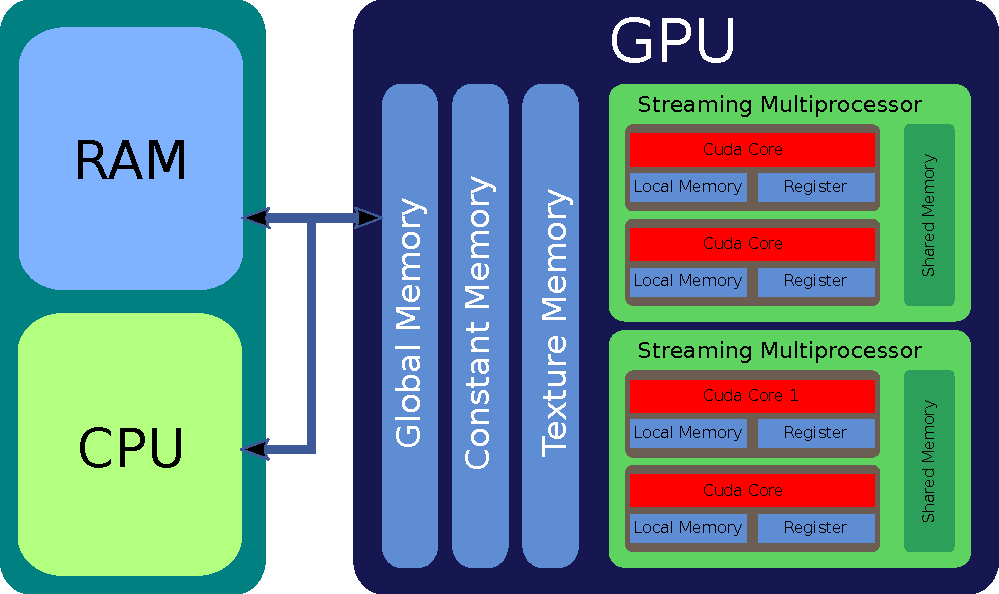
\includegraphics[width=0.9\textwidth]{gfx/cuda/gpu.pdf}
          \caption{Memory layout of a Nvidia-GPU}
    \label{fig:gpu_memory_layout}
\end{figure}

\begin{description}
    \item[Global Memory] The global memory is the largest memory on the GPU and can be accessed by all cuda cores.
                         It is  used to exchange data with the RAM and distribute it between different SMs.
                         Writing and reading from the global memory is slow. A part of the global memory can furthermore be used as a constant memory.
                         In this case multiple memory accesses on the same location are temporary cached.
                         In addition the use of the global memory as a texture memory is possible. The memory access is then spatially cached.


    \item[Shared Memory] Each SM contains a shared memory, much smaller than the global memory \footnote{Around 16kb on c1060 and 64kb on k20m}. It is accessible
                         by all cuda cores of the SM.
                         This memory type is much faster (x100) than the global memory and is usefull when multiple operations
                         by different cuda cores are carried out on the same data.

    \item[Register / Local Memory] Each cuda core posseses an own set of registers and local memory.
                                   The register access is slightly faster than the access  on the shared memory.
                                   Local memory access is very slow since
                                   it is created on the global memory, when the cuda core runs out of resources.
\end{description}

\clearpage

\subsection{Thread Management}
\label{cuda:sec_threadmanage}

In order to distribute the workload between different SMs and cuda cores an additional syntax is necessary.
The CUDA API therefore  introcuces the notion of a thread and a block.

\begin{description}
    \item[Thread] A Thread is the software abstraction of a single cuda core. It can be identified with
                   a maximum of three IDs, \textbf{threadIdx.x}, \textbf{threadIdx.y} and\textbf{threadIdx.z}.

    \item[Block] A block is defined as a group of threads, i.e. in Fig. \ref{cuda:grid_example} a Block contains of 64 threads.
                 There  is no direct hardware equivalent to a block.
                 A block is identified by a maximum of two IDs, \textbf{blockIdx.x} and \textbf{blockIdx.y}

    \item[Blocksize] The blocksize is defined before running a function on the GPU. It determines how
                    many threads run inside a block. In Fig. \ref{cuda:grid_example} the blocksize is set to (8, 8) and
                    each thread has a threadIdx.x and threadIdx.y.

    \item[Gridsize] The gridsize defines the total number of blocks, i.e. (2, 2) in the example.
\end{description}

The concept of a grid containing blocks of threads is a little bit confusing at first.
However these abstractions are necessary to enable a high workload on the GPU,
since each block can be dynamically assigned to a different SM.


\begin{figure}[!bp]
      \centering
        \resizebox{0.5 \textwidth}{!}{
       \import{gfx/cuda//}{grid.pdf_tex}
        }
       \caption{Segmentation of the $y, z$ plane of a simulation domain into a grid of Blocks.
                 Eeach block contains a grid with 8x8 threads.}
       \label{cuda:grid_example}
\end{figure}


\subsection{Performance Considerations}

For the programming of a CUDA device a vast number of optimization techniques exist (see \citep{CUDABP}),
to explain all of these methods would go beyond the scope of this thesis.
Here a short description of the two most import ones is given

\begin{description}
    \item[Memory Coalescing]{
        During the runtime a SM executes a number of 32 threads in parallel, this thread group is denoted as a warp.
        In order to enable a fast memory access on the global memory, all threads in a warp should access
        The global memory should be used for data transfer and distribution, with as little as possible global reads.
        Immediatly after the data is transfered to the shared memory there should be as many as possible computations before transfering
        it back. Furthermore all memory accesses should be optimized}
    \item[Sparse global memory acces]{
        The global memory should be used for data transfer and distribution, with as little as possible global reads.
        Immediatly after the data is transfered to the shared memory there should be as many as possible computations before transfering
        it back. Furthermore all memory accesses should be optimized}
\end{description}


\subsection{Simulation Domain and  Memory Layout}

The three-dimensional simulation domain is given by a cuboid, that is discretized by a
collocated cartesian grid with a constant step size in each direction.
From here on the following conventions will be used.

\begin{description}
    \item[$l_i$] The length of the cube in $x$, $y$ or $z$ direction, $i\in{x, y, z}$
    \item[$N_i$] The number of grid points in $x$, $y$ or $z$ direction, $i\in{x, y, z}$
    \item[$\Delta i$] The stepsize between to grid points in $x$, $y$ or $z$ direction, $i\in{x, y, z}$
\end{description}

A single grid point is determined by the set of indices $i,j,k$ where ${0\leq i < N_x}$,
${0\leq j < N_y}$ and ${0\leq k < N_z}$. The position vector is given by ${\vec{r} = (i\cdot\Delta x, j\cdot \Delta y, k\cdot \Delta z)^T}$.
Each grid point lies in the center of a grid cell of size $\Delta x \cdot \Delta y \cdot \Delta z$,
since a collogated grid is used all variables are located in the cell center.
\footnote{For example on a staggered grid, the velocity components are stored on the cell faces.}
For the computation of a variable $\Phi\in\{v_x, v_y, v_z, \rho\}$ is stored into three registers
\begin{description}
    \item[$C_\Phi$] Located on the RAM. Used mainly for data transfer and analysis
    \item[$R_\Phi$] Located on the global memory on GPU. Here all variables are located after the computation of a time step.
    \item[$B_\Phi$] Located on the global memory on GPU. This is the buffer register for the Williamson RK scheme, see Sec. ().
\end{description}

The size of a storage register is given by $(N_x+4)(N_y+4)(N_z+4)$.
An additional offset $+4$ is given, since two additional layers of ghost points are attached to each side of the simulation domain.
This points are used for a computation of the boundarie conditions, see Sec. ().
All registers contain a one dimensional memory layout.
Hence, the register position of a grid point has to be calculated by

\begin{align}
    P(i, j, k) = i(N_y+4)(N_z+4)+j(N_z+4)+k
\end{align}

which is a row-major access pattern.

\section{Time Step Algorithm}

In this section an overview of the computation of a single time step will be given.
For this example the Navier-Stokes equation given by Eq. \ref{theorie:eqns} will be used.
Before the computation of the time step all initical conditions are saved to the
registers $C_{\Phi}$ and  $R_{\Phi}$.
The time integration is performed with the Willamson-RK3 scheme, see Sec. \ref{numerik:rk_williamson_sec}.
This schemes consist of three sub time step, in this example only the first step given by

\begin{align}
    \begin{split}
    Q_1 = \Delta t \mathcal{L}^*\left(\Phi^n\right)\qquad &\Rightarrow \qquad \Phi^{1} = \Phi^n + \frac{1}{3}Q_1
    \end{split}
\end{align}

will be considered.  The computation of the remaining steps is similar.


The simulation domain is divided into a grid of  $N_y/8 \times N_z/8$ blocks, on each of these the integration is performed separately.
This segmentation is similar to the example introduced in Sec. \ref{cuda:sec_threadmanage} (see Fig. \ref{cuda:grid_example}), except an
additional index threadIdx.z is used.
This index seperates the variables during the integration, i.e. for $v_x$ it is threadIdx.z = 0, for $v_y$  it is 1 and so forth.
With this convention each block contains a total number of 8x8x4 threads.

For a computation of the finite difference schemes  a 5-Point stencil is used, as shown in Fig. \ref{cuda:stencil}.
The inner points of the stencil are enumerated with 1, the outer with 2.. For example in $x$ direction the points are denoted as West2,
West, East2, East in $x$ direction or with the abbreviations W2, W1, E1 and E2.
For second order finite difference schemes, only the inner points  are used, we refer to a 3-Point stencil in this case.

\begin{figure}[!bp]
      \centering
        \resizebox{0.6\textwidth}{!}{
       \import{gfx/cuda//}{stencil.pdf_tex}
        }
        \caption{
            5-Point stencil used for the discretization, with the directions North, West, South, East, Up and Down.
        }
       \label{cuda:stencil}
\end{figure}

\begin{figure}[!bp]
      \centering
        \resizebox{0.6\textwidth}{!}{
       \import{gfx/cuda//}{timestep.pdf_tex}
        }
       \caption{
           Shared memory block location in the simulation domain during a time step.
       }
       \label{cuda:timestep_algo_img}
\end{figure}
\clearpage

The computation of one timestep can be seperated into an initialzation part and a for-loop which iterates by the index $i$, over the simulation domain.
As a first step each thread is assigned to a grid point $(i, j, k)$.

\begin{align}
    \begin{split}
    i &= 2\\
    j &= \text{blockIdx.x}\cdot 8 + \text{threadIdx.y} + 2\\
    k &= \text{blockIdx.y}\cdot 8 + \text{threadIdx.x} + 2
    \end{split}
\end{align}

%The offset 2 is a again result of the ghost points, more on this in Sect. ()
The position of the center $C$ for each thread, is then given by $P(i, j, k)$.
In the next step each thread has to load the neighboor points W2, W1, E1 and E2,
the offset to $C$ is given my a multiple of $L=(N_y+4)(N_z+4)$, for example $W2= C - 2L$.
Furthermore on the sides of the Block two additional points are necessary for the discretization
in the directions U, D, N and S.

With the calculated positions the variables are now loaded into the shared memory of the gpu.
Fig. \ref{cuda:timestep_algo_img} shows how this memory stucture is locatted in the numerical domain, exemplarily for $i>2$.
%Fig (), shows the position in the simulation domain, the 5-Point stencil is exemplariliy shown for one center point,
%furthermore the (ghost?) points on the sides are shown.
The initialization procedure is finished.

In the first step of the for-loop the spatial derivatives are computed.
Since this terms are quite large, here this will be exemplarily shown for the laplace operator
with a central difference scheme of fourth order, given by Eq. \ref{num:fd_o4_methods}, for the $v_x$ component.

\begin{align}
    \begin{split}
    \Delta v_x   \approx &  \frac{1}{12\Delta x^2} \left(-v_x(i+2, j, k) + 16v_x(i+1, j, k) - 30v_x(i, j, k) + 16v_x(i-1, j, k)-v_x(i-2, j, k)\right)\\
                              +&  \frac{1}{12\Delta y^2} \left(-v_x(i, j+2, k) + 16v_x(i, j+1, k) - 30v_x(i, j, k) + 16v_x(i, j-1, k)-v_x(i, j-2, k)\right)\\
                              +&  \frac{1}{12\Delta z^2} \left(-v_x(i, j, k+2) + 16v_x(i, j, k+1) - 30v_x(i, j, k) + 16v_x(i, j, k-1)-v_x(i, j, k-2\right))
    \end{split}
\end{align}

The intermediate step $Q_{\Phi}$ is than computed with the conditionals

\begin{algorithmic}
\IF {(threadIdx.z==0)}
      \STATE ${Q_{\rho} = -\nabla \vec{v}}$
\ENDIF
\IF {(threadIdx.z==1)}
      \STATE ${Q_{v_x} = -(\vec{v} \nabla) v_x - c^2\partial_x\rho + \frac{1}{\Rey}\partial^2_xv_x + \vec{f}_{\text{ext.}}}$
\ENDIF
\IF {(threadIdx.z==2)}
      \STATE ${Q_{v_y} = -(\vec{v} \nabla) v_y - c^2\partial_y\rho + \frac{1}{\Rey}\partial^2_yv_y + \vec{f}_{\text{ext.}}}$
\ENDIF
\IF {(threadIdx.z==3)}
      \STATE ${Q_{v_z} = -(\vec{v} \nabla) v_z - c^2\partial_z\rho + \frac{1}{\Rey}\partial^2_zv_z + \vec{f}_{\text{ext.}}}$
\ENDIF
\end{algorithmic}


stored in new register
The for-loop iterates over the domain by incrementing the $k$ index

\subsection{Boundary Conditions}

For the imlempentation of the boundarie conditions from Sec. () two additional layer of grid points
are added on each side of the simulation domain.
The total number of grid points is ${(N_x + 4)\cdot(N_y + 4)\cdot(N_z + 4)}$.
The additonal points, which are referred to as ghostpoints \citep{ctie},
are computed after each timestep in order to fulfill the boundarie conditions.
For the purpose of explanation we will here consider the one-dimensional case,
for finite differences of fourth order. (The methods were given by atilgner.)

v?

\paragraph{No-Slip Boundaries}\mbox{}\\

The left boundarie is set to the point $b=2$,
the ghost points arg given by $g_2=0$ and $g_1=1$, the inner points close
to the boundarie are $l_1=3$ and $l_2=4$.
In order to obtain No-Slip boundaries the velocity profile is mirrored and inverted
at $b$. Thus, $v(g_2) = -v(l_2)$ and  $v(g_1) = -v(l_1)$



\paragraph{No-Flux and Free-Slip Boundaries}\mbox{}\\

The left boundarie is set to the point $b=2$,
the ghost points arg given by $g_2=0$ and $g_1=1$, the inner points close
to the boundarie are $l_1=3$ and $l_2=4$.
In order to obtain No-Slip boundaries the velocity profile is mirrored and inverted
at $b$. Thus, $v(g_2) = -v(l_2)$ and  $v(g_1) = -v(l_1)$


\paragraph{Periodic Boundaries}\mbox{}\\

The left boundarie is set to the point $b=2$,
the ghost points arg given by $g_2=0$ and $g_1=1$, the inner points close
to the boundarie are $l_1=3$ and $l_2=4$.
In order to obtain No-Slip boundaries the velocity profile is mirrored and inverted
at $b$. Thus, $v(g_2) = -v(l_2)$ and  $v(g_1) = -v(l_1)$

\subsection{Remarks}

-performance blabla
-tilgner bsp
-threads

The position of the points in the shared memory is defined by an offset
The offset of these points to the current one can be computed by

-store date in register

ix wird aufadiert points are shiftet  and the next layer is loaded (img nachtragene)
the procuder is fertig wenn simulation domain  durchgearbetit ist .

\subsection{Boundary Conditions}

For the imlempentation of the boundarie conditions from Sec. () two additional layer of grid points
are added on each side of the simulation domain.
The total number of grid points is ${(N_x + 4)\cdot(N_y + 4)\cdot(N_z + 4)}$.
The additonal points, which are referred to as ghostpoints \citep{ctie},
are computed after each timestep in order to fulfill the boundarie conditions.
For the purpose of explanation we will here consider the one-dimensional case,
for finite differences of fourth order. (The methods were given by atilgner.)

v?

\paragraph{No-Slip Boundaries}\mbox{}\\

The left boundarie is set to the point $b=2$,
the ghost points arg given by $g_2=0$ and $g_1=1$, the inner points close
to the boundarie are $l_1=3$ and $l_2=4$.
In order to obtain No-Slip boundaries the velocity profile is mirrored and inverted
at $b$. Thus, $v(g_2) = -v(l_2)$ and  $v(g_1) = -v(l_1)$



\paragraph{No-Flux and Free-Slip Boundaries}\mbox{}\\

The left boundarie is set to the point $b=2$,
the ghost points arg given by $g_2=0$ and $g_1=1$, the inner points close
to the boundarie are $l_1=3$ and $l_2=4$.
In order to obtain No-Slip boundaries the velocity profile is mirrored and inverted
at $b$. Thus, $v(g_2) = -v(l_2)$ and  $v(g_1) = -v(l_1)$


\paragraph{Periodic Boundaries}\mbox{}\\

The left boundarie is set to the point $b=2$,
the ghost points arg given by $g_2=0$ and $g_1=1$, the inner points close
to the boundarie are $l_1=3$ and $l_2=4$.
In order to obtain No-Slip boundaries the velocity profile is mirrored and inverted
at $b$. Thus, $v(g_2) = -v(l_2)$ and  $v(g_1) = -v(l_1)$

\subsection{Remarks}

-performance blabla
-tilgner bsp
-threads

- measurements / output
- zusammenfassung flow diagramm
- erläuterung threads
- python api

%During execution time each cuda core is executed as a thread, in an SIMD\footnote{Single Instruction Multiple Device}-like behaviour.
%This means every cuda core on one SM executes the same instruction set simultaneously. To differentiate between different cuda cores,
%each get assigned to a different \textbf{ThreadId}.
%With the declaration of a block dimension, we define how many threads are executed in parallel.
%The block dimension can be up to 3-dimensions. In this case each cuda core will be assigned to a ThreadId in x, y and z direction.
%A collection of threads with this grid structure is called a block.
%Since the


